% NOTE: written against the standard \documentclass{llncs} interface used across the
% Springer LNCS/LNNS family. Swap in the exact class/bst files MIDI 2026 links from its
% submission page before final formatting; the content/structure below does not depend on it.
\documentclass[runningheads]{llncs}

\usepackage{graphicx}
\usepackage{booktabs}
\usepackage{amsmath}
\usepackage{hyperref}

\setlength{\textfloatsep}{2mm plus 2pt minus 2pt}
\setlength{\intextsep}{2mm plus 2pt minus 2pt}
\setlength{\belowcaptionskip}{2pt}

\begin{document}

\title{Publication Delay and the Value of Online Adaptation in Monthly Remittance Forecasting}

\author{Samir Murakaev \and Tattybubu Arap kyzy}
\institute{Ala-Too International University, Bishkek, Kyrgyzstan}
\titlerunning{Publication Delay and Online Adaptation in Remittance Forecasting}

\maketitle

\begin{abstract}
Forecasting systems are usually evaluated with complete data, but in operation they adapt using
feedback that arrives late: the outcome needed to score a forecast is published weeks after the
month it describes. We measure how that delay changes the value of adaptation using monthly
remittance inflows to the Kyrgyz Republic -- chosen because in 2022 both the national central bank
and the World Bank projected a large decline that did not materialise, and because a retroactive
redefinition of the series in 2024 provides a second, unplanned natural experiment. We combine
three forecasters -- expanding- and rolling-window ridge regression and a zero-shot time-series
foundation model (Chronos-Bolt) -- with the recursive fixed-share rule, under a chronologically
correct protocol in which every forecast, training row and weight update respects the real
publication calendar reconstructed from 99 archived data versions. We find that models fit on
recent history beat a seasonal-naive benchmark ordinarily but lose to it during the 2022 shock,
that the adaptive combiner recovers only part of naive's shock-period advantage because its own
feedback is itself delayed, and that a definitional break in the target series -- with no
old-definition value for four months, not disentangleable from an ordinary forecasting failure --
degrades every fitted model more than the shock did. A finding that routine, non-adaptive
averaging performs comparably to adaptive weighting is reported as a valid answer, not a null
result to be explained away.
\end{abstract}

\section{Introduction}

Remittances are a large share of household income in the Kyrgyz Republic: personal remittances
received averaged close to 30\% of GDP over 2012--2021. In spring 2022, following the onset of the
war in Ukraine and sanctions on Russia -- source of most of these inflows -- the National Bank of
the Kyrgyz Republic (NBKR) projected a 20\% decline and the World Bank a 32\%. Neither materialised: cumulative inflows
over January--September 2022 exceeded the same period in 2021, and GDP grew by approximately 7\%.
This episode motivates the question studied here, but this study does not attempt to explain the
institutional forecasting error or the behaviour of individual senders.

The underlying computational problem is general. A model is fit on the historical relationship
between predictors and a target; conditions change; the system should adapt, but the evidence that
adaptation is needed is not available immediately -- NBKR's remittance series is published with a
lag of five to eight weeks. The question is therefore not only whether adaptation helps, but
whether it still helps once feedback about \emph{why} it should help arrives late. Two design
decisions follow: adaptation must be evaluated under the real release calendar, not the convenient
assumption that data are available as soon as the month ends, and the comparison must be against a
policy practitioners actually use -- routine retraining and simple averaging -- not a deliberately
weak baseline.

\textbf{Contribution.} None of the three forecasting components is new; the contribution is
methodological and empirical: (i) a chronologically correct evaluation protocol, reconstructed
from 99 archived data versions rather than assumed, with an automated test suite (1{,}553 checks)
verifying the absence of look-ahead leakage; (ii) a measurement of how much of adaptive
combination's advantage survives this delay, including a stress test built around a retroactive
target redefinition we did not anticipate when the study was designed; and (iii) we are not aware
of prior work evaluating a zero-shot time-series foundation model as one voice in an
online-aggregated ensemble under delayed feedback, rather than as a standalone baseline.

\section{Related Work}

\textbf{Forecast combination and estimation windows.} Combining forecasts is long
established~\cite{bates1969combination,timmermann2006forecast}; under structural change, switching
or averaging across estimation windows of different length is a known
strategy~\cite{pesaran2007selection}, and Rossi~\cite{rossi2021forecasting} surveys forecasting
under instability. Combining experts with weights updated from observed losses is a mature field:
exponentially weighted averaging~\cite{cesabianchi2006prediction}, the fixed-share rule for
tracking a changing best expert~\cite{herbster1998tracking}, and polynomially weighted variants
such as ML-Poly~\cite{gaillard2014second}, implemented in \texttt{opera}~\cite{opera}.

\textbf{Delayed feedback and real-time evaluation.} The data-stream literature studies learning
when labels arrive late (\emph{verification latency}~\cite{gama2014survey}); delayed and optimistic
online learning has formal regret guarantees~\cite{joulani2013online,flaspohler2021online},
including a subseasonal-climate application~\cite{flaspohler2021online} sharing our motivation. We
differ in using fixed monthly lags on a short macroeconomic series and evaluating combination
rules already used in practice
rather than proposing new regret-optimal algorithms. Macroeconomic forecasting has long
distinguished evaluation on revised data from data actually available at the
time~\cite{croushore2001realtime}, rarely applied to remittance forecasting, where published
studies typically use the latest revised series.

\textbf{Model complexity and TSFMs.} For short monthly series we favour strong simple baselines
over deep sequence models trained from scratch, consistent with evidence that linear baselines
remain competitive with deep architectures on forecasting benchmarks~\cite{zeng2023transformers}.
Pretrained time-series foundation models (TSFMs) such as Chronos~\cite{ansari2024chronos} and
Lag-Llama~\cite{rasul2023lagllama} sidestep this risk by forecasting zero-shot. The closest prior
work~\cite{jetwiriyanon2025tsfmecon} finds TSFMs match classical models in stable conditions but
degrade during shocks; we find a consistent pattern (Section~\ref{sec:results}) under a materially
different protocol -- chronologically correct, delayed-publication, combining the TSFM with other
experts online rather than evaluating it standalone (pretraining-corpus contamination risk
discussed in Section~\ref{sec:limitations}).

\section{Data and Real-Time Protocol}
\label{sec:data}

The target is monthly cross-border remittance inflows to the Kyrgyz Republic in US dollars, as
published by NBKR. We reconstruct what a forecaster could have known at each historical issue date
from 99 versions of NBKR's published table, recovered from the NBKR website and the Internet
Archive (2015-12-16 to the latest release). Two facts about this archive shape the protocol.

First, publication lag is consistently five to eight weeks (35--54 days, median 41): the value for
month $m$ is not published until well into month $m+1$, and is reliably available by month $m+2$.
We take month $m$ to be \emph{known} at issue date $v$ once it appears in the archived vintage most
recently published on or before $v$, or -- for the small number of gaps our crawl missed -- in the
earliest vintage reporting it under the same accounting definition as the vintage current at $v$
(defined next). Within-definition revisions are small: at a materiality threshold of \$0.02
million (below the source spreadsheets' rounding resolution), 9 of 97 consecutive vintage pairs
revise any shared month at all, by less than 4\% in all but one case; counting any nonzero float
difference instead gives 12, three sub-threshold.

Second, in a vintage dated 2024-02-14, NBKR redefined the series -- from transfers through
money-transfer systems to all cross-border instruments, including mobile banking and e-wallets --
retroactively to 2022 onward, with revisions of up to 66\% for individual months. We treat this as
a first-class fact rather than noise: a forecaster issuing a forecast in December 2023 could not
have known the target's own definition would change four months later. October 2023 -- January
2024 were never published under the old definition at all, so no historically consistent value
exists for these months under either definition, and we do not attempt to construct one.

\textbf{Ground truth.} The evaluation target for month $m$ is its \emph{first release} rather than
the latest, most-revised value: scoring against the latest value would require predicting a
methodological change made two years later. First-release and latest values coincide to within
revision noise outside the 2023--24 window. \textbf{Leakage testing:} the real-time information
function is tested against 1{,}553 automated pytest checks, including that no forecast origin
observes any month past its true publication cutoff and, for all 227 issue dates before
2024-02-14, that no value reaching the forecaster is sourced from a post-redefinition vintage. All
tests pass.

\begin{figure}[t]
\centering
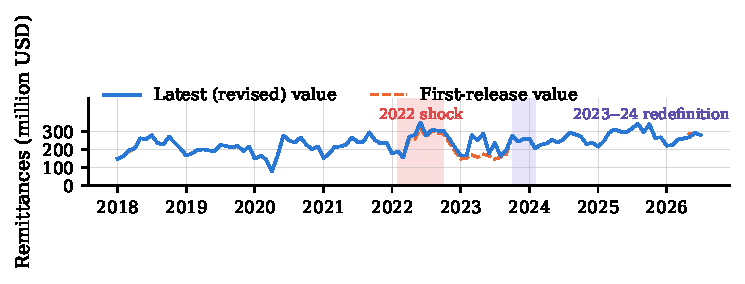
\includegraphics[width=\linewidth]{figures/fig1_series.pdf}
\caption{Monthly remittance inflows, 2018--2026: latest (revised) vs.\ first-release values. The
2022 shock shows no decline in either series; the 2023--24 redefinition opens a persistent gap
between first-release and latest values.}
\label{fig:series}
\end{figure}

\section{Methodology}
\label{sec:methodology}

Forecasts are issued at the end of each month $v$ for target month $t = v+1$ (horizon $h=1$).
E1 and E2 are fit on $z_t = \log y_t$; their point forecast is $\hat y = \exp(\hat z)$, the
conditional median of $y_t$ under a symmetric error distribution for $z_t$. E3 (below) is not
log-transformed -- it is given the series in levels, its native input scale.

\textbf{Lag choice.} E1/E2 share predictors $z_{t-1}$, $z_{t-2}$, $z_{t-3}$, $z_{t-12}$ (short-run
momentum plus year-over-year seasonality) and eleven monthly indicators, fixed a priori rather
than grid-searched like $\alpha$, $w$ and the fixed-share hyperparameters below. A post hoc,
development-only check against seven alternatives finds a marginally better set, $\{1,3,6,12\}$
(6.3\%/2.7\% lower development MAE for E1/E2) -- on the order of the shock-window bootstrap noise
in Section~\ref{sec:results}; we keep the frozen set rather than re-tuning the pipeline for a
difference this small.

\textbf{E1 -- Expanding ridge.} Ridge regression, refit at every issue date on all months whose
predictors are fully known at $v$, using the training set growing from the start of the series.
$\alpha \in \{0.01, 0.03, 0.1, 0.3, 1, 3, 10, 30, 100\}$ was grid-searched on the development
period alone; $\alpha=0.1$ chosen.

\textbf{E2 -- Rolling ridge.} The same specification, refit at every issue date on only the most
recent $w$ eligible rows. Window $w \in \{24, 36, 48\}$ and, separately, $\alpha$ (same grid as E1)
were each selected on the development period alone; $w=48$, $\alpha=1$ chosen (E1/E2 differ in
$\alpha$ because training-set size, and the bias-variance trade-off it corrects for, differs by
construction).

\textbf{E3 -- Chronos-Bolt (zero-shot).} At each issue date, pretrained Chronos-Bolt-small
\cite{ansari2024chronos} (HF Hub revision \texttt{772f3d2}, pinned) is given the same
real-time-eligible history as E1/E2, in levels, and asked for a one-step-ahead forecast; the
predicted median is the point forecast. No parameters are fit on our data.

\textbf{Combination.} The three experts, plus a seasonal-naive reference (repeat month $t-12$),
are combined with the recursive fixed-share rule~\cite{herbster1998tracking}:
\begin{align}
q_{k,n} &= \frac{p_{k,n-1}\exp(-\eta\,\ell_{k,n})}{\sum_j p_{j,n-1}\exp(-\eta\,\ell_{j,n})}, &
p_{k,n} &= (1-\alpha)\,q_{k,n} + \frac{\alpha}{K}, \quad K=4,
\end{align}
where $\ell_{k,n} = \min(|\hat y_{k,n} - y_n| / c,\ 1)$ is a clipped loss and $n$ indexes
\emph{feedback events}: an outcome for month $m$ is eligible to update weights only once known
under Section~\ref{sec:data}'s protocol, so a weight update at $v$ typically uses feedback from
roughly three months earlier, not the immediately preceding month. Hyperparameters $\eta=0.5$,
$\alpha=0.05$ and the loss-clipping constant $c=74.66$ (95th percentile of pooled absolute errors)
were grid-searched on the development period only and never re-estimated; weights start uniform.
\textbf{Baselines:} seasonal
naive; expanding ridge alone (routine retraining); equal-weight averaging of all four candidates
with no adaptation; the tuned fixed-share combination.

\section{Evaluation Plan}

Development runs through 2021-12 (window/hyperparameter selection only); evaluation issue dates
run 2022-01-31 through 2026-06-30, 54 origins, of which the most recent lacks a known outcome and
is excluded (53 origins with ground truth). Three overlapping windows are reported: the \emph{main
window} excludes the four redefinition-transition months (2023-10 through 2024-01, $n=49$); the
\emph{shock window} is the eight 2022-02 through 2022-09 target months ($n=8$), a subset of the
main window; the \emph{transition window} is the four excluded months ($n=4$), reported
descriptively only. The primary metric is MAE in millions of USD, chosen for direct
interpretability~\cite{hyndman2006another}. Uncertainty on paired differences is summarised by a
paired moving-block bootstrap over origins (5{,}000 resamples), with block lengths 3, 6 and 12
months reported as a sensitivity; at $n=8$ these give 6, 3 and 1 valid block-start positions, so
the 12-month block is degenerate and even the 3-month block draws from a coarse grid, stated
wherever a shock-window interval is reported. No test of conditional predictive ability is
reported since its assumptions are undemonstrated here; non-significance is never presented as
evidence of equivalence.

\section{Results}
\label{sec:results}

\subsection{Adaptation reverses during the shock}

\begin{table}[t]
\centering
\caption{MAE (million USD) by evaluation window. Shock is a subset of Main, not a disjoint slice;
Full equals the weighted average of Main and the separately reported Transition window.}
\label{tab:expert-race}
\resizebox{\linewidth}{!}{%
\begin{tabular}{lcccc}
\toprule
Expert & Main ($n{=}49$) & Shock ($n{=}8$) & Transition ($n{=}4$) & Full ($n{=}53$)\\
\midrule
Seasonal naive        & 49.0 & \textbf{35.3} & 49.3  & 49.0 \\
Expanding ridge (E1)   & \textbf{32.7} & 53.4 & 115.6 & \textbf{38.9} \\
Rolling ridge, $w{=}48$ (E2) & 35.8 & 52.7 & 96.2  & 40.3 \\
Chronos zero-shot (E3) & 37.7 & 42.7 & 87.6  & 41.5 \\
\bottomrule
\end{tabular}%
}
\end{table}

Table~\ref{tab:expert-race} shows the central empirical pattern. Outside the shock, models fit on
recent history are markedly more accurate than the seasonal-naive benchmark -- expanding ridge is
nearly 1.5$\times$ more accurate on the main window. During the eight-month 2022 shock this
reverses: every fitted model is less accurate than naive, and expanding ridge, with the longest
memory, is least accurate of all -- the same mechanism that misled the two institutional
forecasters: a model extrapolating a recent trend is worst off exactly when that trend reverses.

The transition window makes the mechanism starker: naive is nearly unaffected (49.3, close to its
usual level), while the three fitted models are two to three times worse than even the 2022 shock
(87.6--115.6 vs.\ 42.7--53.4). Because October 2023 -- January 2024 was never published under the
old definition (Section~\ref{sec:data}), this large error cannot be cleanly separated into a
forecasting failure and a measurement artefact. We report it as such rather than attributing it to
either cause: a forecaster trained honestly in real time is not protected against its target's own
definition changing retroactively without warning, and that is the object of this stress test, not
a limitation of it.

\begin{figure}[t]
\centering
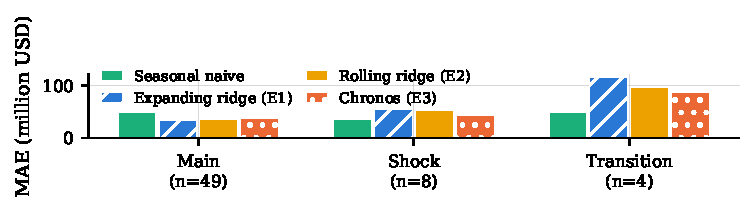
\includegraphics[width=\linewidth]{figures/fig2_mae_by_window.pdf}
\caption{MAE by expert and window (Table~\ref{tab:expert-race}). Naive is worst on Main but best
on Shock; every fitted model reverses along with it.}
\label{fig:mae-bars}
\end{figure}

\subsection{Does the adaptive combiner recover the lost ground?}

\begin{table}[t]
\centering
\caption{Fixed-share vs.\ equal-weight, MAE (million USD), with paired moving-block bootstrap 95\%
CIs on the difference (positive = fixed-share worse); block length 3 for the shock window.}
\label{tab:fs-vs-eq}
\small
\begin{tabular}{lcc}
\toprule
 & Main window ($n{=}49$) & Shock ($n{=}8$) \\
\midrule
Fixed-share      & 35.93 & 45.59 \\
Equal-weight     & 34.62 & 44.16 \\
Bootstrap 95\% CI on difference & $[-0.29, +2.34]$ & $[+0.29, +2.15]$ \\
\bottomrule
\end{tabular}
\end{table}

On the main window (Table~\ref{tab:fs-vs-eq}) the point estimate favours equal-weight, but the
interval includes zero: adaptive weighting is not distinguishable from non-adaptive averaging in
the ordinary period. Within the shock window the gap is bootstrap-significant at every
non-degenerate block length, but $n=8$ is small and the 12-month block is degenerate by
construction; we treat this as suggestive, not conclusive.

The comparison is asymmetric: the same bootstrap against naive on the shock window gives $+10.2$
(95\% CI $[+1.9, +20.4]$, robust even at the coarse 3-month block), but against Chronos only
$+2.9$ (95\% CI $[-7.4, +12.7]$, including zero) -- fixed-share reliably underperforms naive during
the shock but is not reliably distinguishable from its best individual component, Chronos.

The mechanism is visible in the weight trajectory: naive's weight moves from 0.220 in February
2022 to only 0.294 by September, recognising its advantage too slowly to help during the most
acute months (April--June); the delay is sharper in the transition window, where naive's weight
\emph{falls} from 0.178 (October) to 0.117 (December 2023) -- away from, not toward, the
best-performing expert -- then sits unchanged between December and January, when the combiner's
own feedback was itself delayed by the redefinition: the same delay that motivates the study can
disable its own feedback loop exactly when fast adaptation is most valuable.

\subsection{Robustness checks}

Adding $k \in \{1,2,3\}$ months of artificial delay on top of the natural publication lag (Experiment D), with $\eta,\alpha$ fixed at their development-tuned values, changes main-window MAE by
at most $0.21$ (bootstrap CIs all include zero): under the tuned, conservative $\eta=0.5$, the
combiner reacts slowly enough that extra delay adds little on top of the natural $\sim$3-month lag.
Setting $\alpha=0$ (no weight floor) instead improves main-window MAE to 33.3 (from 35.9) but
worsens shock-window MAE to 53.0 (from 45.6): naive and Chronos are driven to weights below 0.02
during development and cannot recover once they begin winning; $\alpha=0.05$ lets both retain
enough weight to partially benefit from a reversal -- the standard stability-plasticity trade-off,
and why development tuning (which includes its own shock, COVID-19 2020) selects non-zero $\alpha$
over the point estimate that otherwise looks best on average.

\section{Limitations}
\label{sec:limitations}

\textbf{No causal claims; small-sample inference.} This is a forecast-accuracy comparison, not a
causal one. The shock window has 8 origins and the transition window 4; the latter is reported
descriptively only, without a CI, and an absent interval should not be read as an absent effect.
Bootstrap intervals on the shock window are sensitive to block length; reported with that caveat,
not as a single number.

\textbf{Multiple comparisons.} Section~\ref{sec:results} reports seven pairwise 95\% bootstrap
intervals without a multiplicity correction (naive Bonferroni: family-wise error up to
$1-0.95^7\approx30\%$); we do not correct because the comparisons share data and overlapping
windows and are not independent, which would make Bonferroni overly conservative the other way.
The one interval excluding zero outside the pre-registered comparison (fixed-share vs.\ naive,
shock window) matches the paper's predicted mechanism -- evidence against a multiplicity artifact,
not proof.

\textbf{TSFM pretraining exposure; definitional discontinuity.} We cannot rule out Chronos's
pretraining corpus containing series correlated with 2022 macroeconomic conditions; its errors are
directionally similar to the institutional forecasters' (underestimating the recovery), evidence
against gross contamination but not proof of its absence. The transition-window error similarly
mixes forecasting failure and measurement discontinuity in a way the data cannot separate; we
report both readings rather than choosing one.

\textbf{Scope.} Results are specific to this series, period and model families; deep sequence
models were not evaluated, and covariates (FX, oil prices) were excluded because their own
publication lags could not be aligned with the horizon without a separate leakage risk.

\section{Conclusion}

Using a chronologically correct protocol validated against 1{,}553 automated leakage checks, we
find that the accuracy advantage of models fit on recent history over a seasonal-naive benchmark
reverses during an economic shock, that adaptive online combination recovers only part of that
reversal because its own feedback is delayed by the same publication lag the study is about, and
that a retroactive redefinition of the target variable is at least as damaging to every fitted
model as the shock itself -- while being, in part, not a forecasting problem at all. A finding
that simple equal-weight averaging performs comparably to a tuned adaptive combiner is reported as
an answer to the research question, not a failure to find one.

\bibliographystyle{splncs04}
\bibliography{refs}

\end{document}
